\documentclass{sig-alternate}
%\documentclass{lms}
\usepackage[utf8]{inputenc}

\usepackage{amsmath,amssymb}
\usepackage{amsrefs}
\usepackage[usenames,dvipsnames]{color}
\usepackage{stmaryrd}
\usepackage{enumerate}
\usepackage[algoruled,vlined,english,linesnumbered]{algorithm2e}
\usepackage[pdfpagelabels,colorlinks=true,citecolor=blue]{hyperref}
\usepackage{comment}
\usepackage{tikz}
\renewcommand*{\theHsection}{\thesection}

\newcommand{\noopsort}[1]{}
\DeclareMathOperator{\NP}{NP}
\DeclareMathOperator{\GL}{GL}
\DeclareMathOperator{\val}{val}
\DeclareMathOperator{\pr}{pr}
\DeclareMathOperator{\tr}{Tr}
\DeclareMathOperator{\com}{Com}
\DeclareMathOperator{\Grass}{Grass}
\DeclareMathOperator{\Lat}{Lat}
\DeclareMathOperator{\round}{round}

\begin{document}

\newtheorem{theo}{Theorem}[section]
\newtheorem{lem}[theo]{Lemma}
\newtheorem{prop}[theo]{Proposition}
\newtheorem{cor}[theo]{Corollary}
\newtheorem{quest}[theo]{Question}
%\theoremstyle{definition}
\newtheorem{rem}[theo]{Remark}
\newtheorem{ex}[theo]{Example}
\newtheorem{deftn}[theo]{Definition}
\newtheorem{rmk}[theo]{Remark}

\newcommand{\N}{\mathbb N}
\newcommand{\Z}{\mathbb Z}
\newcommand{\Zp}{\Z_p}
\newcommand{\Q}{\mathbb Q}
\newcommand{\Qp}{\Q_p}
\newcommand{\Fp}{\mathbb{F}_p}
\newcommand{\R}{\mathbb R}
\renewcommand{\O}{\mathcal O}
\newcommand{\OK}{\mathcal{O}_K}
\newcommand{\XX}{\mathbf X}
\newcommand{\trans}{{}^{\text t}}
\newcommand{\T}{\mathcal{T}}

\renewcommand{\prec}{\text{\rm prec}}

\newcommand{\id}{\textrm{id}}
\newcommand{\Epi}{\textrm{Epi}}

\newcommand{\lb}{\ensuremath{\llbracket}}
\newcommand{\rb}{\ensuremath{\rrbracket}}
\newcommand{\lp}{(\!(}
\newcommand{\rp}{)\!)}
\newcommand{\col}{\: : \:}

\def\todo#1{\ \!\!{\color{red} #1}}
\definecolor{purple}{rgb}{0.6,0,0.6}
\def\todofor#1#2{\ \!\!{\color{purple} {\bf #1}: #2}}

\def\binom#1#2{\Big(\begin{array}{cc} #1 \\ #2 \end{array}\Big)}

\title{Tracking p-adic precision: examples}

\numberofauthors{3}
\author{
\alignauthor Xavier Caruso\\
  \affaddr{Universit\'e Rennes 1}\\
  \email{\normalsize \textsf{xavier.caruso@normalesup.org}}
\alignauthor Tristan Vaccon\\
  \affaddr{Universit\'e Rennes 1}\\
  \email{\normalsize \textsf{tristan.vaccon@univ-rennes1.fr}}
\alignauthor David Roe \\
  \affaddr{University of Calgary}\\
  \email{\normalsize \textsf{roed.math@gmail.com}}
}

\maketitle

\begin{abstract}
\end{abstract}

\vspace{1mm}
 \noindent
 {\bf Categories and Subject Descriptors:} \\
\noindent I.1.2 [{\bf Computing Methodologies}]:{~} Symbolic and Algebraic
  Manipulation -- \emph{Algebraic Algorithms}

 \vspace{1mm}
 \noindent
 {\bf General Terms:} Algorithms, Theory

 \vspace{1mm}
 \noindent
 {\bf Keywords:} 
\medskip

\section{Introduction}

\section{Preliminaries}

In the next section, we will see that the derivative at some point $x$ 
of many standard operations, modelised by a function $f$, has a simple 
expression in term of $x$ and $f(x)$. In other terms, such functions $f$
satisfy:
\begin{equation}
\label{eq:diffequa}
f' = g \circ (f, \id)
\end{equation}
where $g$ is a given --- and hopefully rather simple --- function. 
The aim of these preliminaries is to study the differential equation
\eqref{eq:diffequa} (or, actually, a slight generalization of it) and
to derive from it some bounds on the growing function $\Lambda(f)$ 
defined in \cite{padicprec}.

\emph{In all this section, we assume that \textbf{the base field $K$ 
has characteristic $0$}.}

\begin{comment}

\subsection{Legendre transform of a compositum}

For $i \in \{1,2\}$, let $\varphi : \R \to \R \cap \{+\infty\}$ denote a 
convex function and $\varphi_i^\star$ be its Legendre transform defined 
by:
\begin{equation}
\label{eq:defLegendre}
\varphi_i^\star(u) = \sup_{v \in \R} \varphi(v) - uv.
\end{equation}
Set $\varphi = \varphi_1 \circ \varphi_2$. The aim of this subsection is 
to relate $\varphi^\star$ with $\varphi_1^\star$ and $\varphi_2^\star$.

\begin{lem}
\label{lem:Legendrecomp}
We assume that $\varphi_1$ and $\varphi_2$ are nondecreasing and that 
their slopes are all in $\N$. Then, for all nonnegative interger $s$:
$$\varphi^\star(s) =
\inf_{\ell, (n_i)} \varphi_1^\star(\ell) + \varphi_2^\star(n_1) + 
\cdots + \varphi_2^\star(n_\ell)$$
where the infimum is taken over all finite sequences of nonnegative
integers (of variable length) $n_1, \ldots, n_\ell$ with $n_1 + \cdots +
n_\ell = s$.
\end{lem}

\begin{proof}
Let $n_1, \ldots, n_\ell$ be a sequence as above. Taking the supremum 
in $v$ in the relation:
$$\varphi(v) - s v =
\varphi_1(\varphi_2(v)) - \ell \varphi_2(v) + \sum_{i=1}^\ell
(\varphi_2(v) - n_i v)$$
we get:
\begin{equation}
\label{eq:inegvarphi}
\varphi^\star(s) \leq \varphi_1^\star(\ell) + 
\varphi_2^\star(n_1) + \cdots + \varphi_2^\star(n_\ell).
\end{equation}
It remains then to prove that one can choose $\ell$ and $n_1, \ldots,
n_\ell$ such that the inequality above is actually an equality.

Let $x$ be the unique value such that the left (resp. right) derivative 
of $\varphi$ at $x$ is less than (resp. greater than) or equal to $s$. 
Let $\ell^-$ (resp. $\ell^+$) denote the left (resp. right) derivative 
of $\varphi_1$ at $\varphi_2(x)$ and $n^-$ (resp. $n^+$) denote the left 
(resp. right) derivative of $\varphi_2$ at $x$. On the one hand, $\ell^- 
n^- \leq s \leq \ell^+ n^+$ since $\ell^- n^-$ (resp. $\ell^+ n^+$) 
equals the left (resp. right) derivative of $\varphi$ at $x$). On the 
other hand:
$$\begin{array}{ll}
\varphi_1^\star(u) = \varphi(x) - u \varphi_2(x) & 
\text{for all } u \in [\ell^-,\, \ell^+] \\
\varphi_2^\star(u) = \varphi_2(x) - u x & 
\text{for all } u \in [n^-,\, n^+] \\
\varphi^\star(u) = \varphi(x) - u x & 
\text{for all } u \in [\ell^- n^-,\, \ell^+ n^+] \\
\end{array}$$
Therefore, the inequality \eqref{eq:inegvarphi} is an equality for all 
integer $\ell \in [\ell^-, \ell^+]$ and all sequences of integers 
$(n_i)_{1 \leq i \leq \ell}$ with $n_i \in [n^-, n^+]$ for all $i$ and 
$n_1 + \cdots + n_\ell = s$. It is then enough to prove that such a 
couple $(\ell, (n_i))$ exists but it is clear.
\end{proof}

\end{comment}

\subsection{Composite of locally analytic functions}

Let $U$, $V$ and $W$ be three open subsets is some $K$-Banach spaces 
$E$, $F$ and $G$ respectively. We assume that $0 \in U$, $0 \in V$. Let 
$f : U \to V$ and $g : V \to W$ be two locally analytic functions around 
$0$ with $f(0) = 0$. The composition $h = g \circ f$ is then locally 
analytic around $0$ as well. Let us write the analytic expansion of $f$, 
$g$ and $h$ as follows:
$$f = \sum_{n \geq 0} f_n, \quad 
g = \sum_{n \geq 0} g_n, \quad
h = \sum_{n \geq 0} h_n, \quad$$
where $f_n$, $g_n$ and $h_n$ are the restrictions to the diagonal of 
some symmetric $n$-linear forms $F_n$, $G_n$ and $H_n$ respectively. The 
aim of this subsection is to prove the following proposition.

\begin{prop}
\label{prop:boundhr}
With the above notations, we have for all nonnegative integer $r$:
$$\Vert h_r \Vert \leq \sup_{m, (n_i)}
  \Vert g_m \Vert \cdot \Vert f_{n_1} \Vert \cdots \Vert f_{n_m} \Vert$$
where the supremum is taken over all couples $(m, (n_i))$ where $m$
is a nonnegative integer and $(n_i)_{1 \leq i \leq m}$ is a sequence of
length $m$ of nonnegative integers such that $n_1 + \ldots + n_m = r$.
\end{prop}

During the proof, multinomial coefficients will play an important role. 
We recall that they are defined as follows: 
given $s, k_1, \ldots, k_\ell$ some positive integers with $s \geq
k_1 + \cdots + k_\ell$, we set:
$$\binom s {k_1 \,\, k_2 \,\, \cdots \,\, k_\ell} =
  \frac{s!}{k_1!\: k_2! \cdots k_\ell! \: (s{-}k_1{-}\cdots{-}k_\ell)!}.$$
We also recall that these numbers are all positive integers.

We now expand $g \circ f$ as follows:
\begin{align}
g \circ f & = \sum_{m \geq 0} g_m \Big(\sum_{n \geq 1} f_n\Big) \nonumber \\
& = \sum \binom m {\!k_1 \,\, \cdots \,\, k_\ell\!} \:
G_m(f_{n_1}, \ldots, f_{n_1}, \ldots, f_{n_\ell}, \ldots, f_{n_\ell})
\label{eq:expansiongf}
\end{align}
where the latest sum runs over:

\noindent
(a) all finite sequences $(k_i)$ of positive integers whose length 
(resp. sum) is denoted by $\ell$ (resp. $m$), and

\noindent
(b) all finite sequences $(n_i)$ of positive integers of length
$\ell$.

\noindent
Moreover, in the argument of $G_m$, the variable $f_{n_i}$ 
is repeated $k_i$ times.

The degree of $G_m(f_{n_1}, \ldots, f_{n_1}, \ldots, f_{n_\ell},
\ldots, f_{n_\ell})$ is $r = k_1 n_1 + \ldots + k_\ell n_\ell$ and 
then contributes to $h_r$. As a consequence $h_r$ is equal to 
\eqref{eq:expansiongf} where the sum is restricted to sequences
$(k_i)$, $(n_i)$ such that $k_1 n_1 + \ldots + k_\ell n_\ell = r$.
Proposition \ref{prop:boundhr} now follows from the next lemma.

\begin{lem}
Let $\mathcal E$ be a $K$-vector space. Let $\varphi : \mathcal E^n \to 
K$ be a symmetric $s$-linear form and $\psi: E \to K$ defined by 
$\psi(x) = \varphi(x, x, \ldots, x)$.
Given $k_1, \ldots, k_\ell$ some positive integers whose sum is $m$ and 
$x_1, \ldots, x_\ell$ some elements of $\mathcal E$, we have:
$$\begin{array}{l}
\Big\Vert \binom m {k_1 \,\, k_2 \,\, \cdots \,\, k_\ell} \cdot
\varphi(x_1, \ldots, x_1, \ldots, x_\ell, \ldots,
x_\ell) \Big\Vert  \\
\hspace{4.3cm} \leq \Vert \psi \Vert \cdot \Vert x_1 \Vert^{k_1} \cdots
 \Vert x_\ell \Vert^{k_\ell}
\end{array}$$
where, in LHS, the variable $x_i$ is repeated $k_i$ times.
\end{lem}

\begin{proof}
It is enough to prove that:
\begin{equation}
\label{eq:normpolar}
\Big\Vert \binom m {k_1 \,\, k_2 \,\, \cdots \,\, k_\ell} \cdot
\varphi(x_1, \ldots, x_1, \ldots, x_\ell, \ldots,
x_\ell) \Big\Vert \leq \Vert \psi \Vert
\end{equation}
provided that all the $x_i$'s have norm at most $1$. We proceed by 
induction on 
$\ell$. If $\ell = 1$, Eq.~\eqref{eq:normpolar} follows directly from
the definition of $\Vert \psi \Vert$. 
We now pick $(\ell+1)$ integers $k_1, \ldots, k_{\ell+1}$ whose sum 
equals $m$ together with $(\ell+1)$ elements $x_1, \ldots, x_{\ell+1}$
lying in the unit ball of $\mathcal E$.
We also consider a new variable $\lambda$ varying in
$\O_K$. We set $x'_i = x_i$, $k'_i = k_i$ when $i < \ell$ and $x'_\ell 
= x_\ell + \lambda x_{\ell+1}$, $k'_\ell = k_\ell + k_{\ell+1}$. By the 
induction hypothesis, we know that the inequality:
$$\Big\Vert \binom s {k'_1 \,\, \cdots \,\, k'_\ell} \cdot
\varphi(x'_1, \ldots, x'_1, \ldots, x'_\ell, \ldots, x'_\ell) \Big\Vert
\leq \Vert \psi \Vert$$
holds for all $\lambda \in K$. Furthermore, LHS of the above inequality
is a polynomial $P(\lambda)$ of degree $k'_\ell$ whose coefficient in 
$\lambda^j$ is:
$$\binom s {k'_1 \,\, \cdots \,\, k'_\ell} \cdot
\binom {k'_\ell} {j} \cdot
\varphi(\underline x_j) = 
\binom s {k_1 \,\, \cdots \,\, k_{\ell-1} \,\, j} \cdot
\varphi(\underline x_j)$$
with
$$\underline x_j = (x_1, \ldots, x_1, \ldots, x_{\ell+1}, \ldots, 
x_{\ell+1})$$
where $x_i$ is repeated $k_i$ times if $i < \ell$ and $x_\ell$ 
(resp. $x_{\ell+1}$) is repeated $j$ times (resp. $k'_\ell - j$ times).
Since $\Vert P(\lambda) \Vert \leq \Vert \psi \Vert$ for all $\lambda$ in 
the unit ball, the norm of all its coefficients must be at most $\Vert \psi
\Vert$ as well. Looking at the coefficient in $\lambda^{k_{l+1}}$, we find
Eq.~\eqref{eq:normpolar} for the families $(k_1, \ldots, k_{\ell+1})$ 
and $(x_1, \ldots, x_{\ell+1})$. The induction follows.
\end{proof}

\subsection{Bounding a growing function}
\label{ssec:boundLambdaf}

We now study a slight generalization of the differential equation 
\eqref{eq:diffequa}, which is:
\begin{equation}
\label{eq:diffequah}
f' = g \circ (f, h).
\end{equation}
Here $g$ and $h$ are known locally analytic functions and $f$ is the 
unknown, which is assumed to be locally analytic as well. The function
$f$ goes from $U$ to $V$, two open subsets in $K$-Banach spaces $E$ 
and $F$ respectively. The function $h$ goes from $U$ to $W$ where $W$
is again an open subset in a $K$-Banach space $G$. Consequently, $g$
goes from $V \times W$ to the vector space $\mathcal L(E,F)$ gathering
all continuous linear applications $E \to F$.
In what follows, we always assume that $V$ and $W$ contains the origin, 
$f(0) = 0$, $h(0) = 0$ and $g(0) \neq 0$. There assumptions are harmless 
because (1)~we can always shift $f$ and $h$ (and $g$ accordingly) so 
that they both vanish at $0$ and (2)~in order to apply the theory of 
\cite{padicprec}, the derivative $f'(0)$ needs to be surjective and 
therefore \emph{a fortiori} nonzero.

Let us write the analytic expansion of $f$, $g$ and $h$ as follows: 
$$f = \sum_{n \geq 0} f_n, \quad
g = \sum_{n \geq 0} g_n, \quad
h = \sum_{n \geq 0} h_n$$
where $f_n$, $g_n$ and $h_n$ are the restrictions to the diagonal of 
some symmetric $n$-linear forms $F_n$, $G_n$ and $H_n$ respectively.
Following \cite{padicprec}, we define $\NP(f) : \R \to \R \cup 
\{+\infty\}$ as the greatest convex function such that $\NP(f)(n) \geq - 
\log \Vert f_n \Vert$ for all integer $n$ and denote by $\Lambda(f)$ its 
Legendre transform. We define $\NP(g)$, $\Lambda(g)$, $\NP(h)$ and
$\Lambda(h)$ similarly.

We consider a nonnegative real number $\alpha$ such that $\Vert n! \Vert 
\geq e^{-\alpha n}$ for all positive integer $n$. A suitable value for 
$\alpha$ is
$$\alpha = - \frac p {p-1} \cdot \log \Vert p \Vert > 0$$
where $p$ denotes the characteristic of the residue field and
where, by convention, the above expression equals $0$ if $p = 0$
(we recall that we have assumed that $K$ has characteristic $0$).

\begin{prop}
\label{prop:boundLambdaf}
We keep the above notations. If the couple $(a,b)$ satisfies:
\begin{equation}
\label{eq:condAB}
b \geq a + \Lambda(g)\big( \! \max(b, \, \Lambda(h) (a)) \big)
\end{equation}
then $b \geq \Lambda(f)(a - \alpha)$.
\end{prop}

\begin{proof}
We have $f' = \sum_{n \geq 0} f'_n$ where
$$f'_n : U \to \mathcal L(E,F), \quad
x \mapsto \big(h \mapsto n \cdot F_n(h, x, x, \ldots, x)\big).$$
In particular, taking $h = x$, we find:
\begin{equation}
\label{eq:normderivative}
\Vert f'_n \Vert \geq \Vert n f_n \Vert = 
\Vert n \Vert \cdot \Vert f_n \Vert.
\end{equation}
Combining this with Proposition \ref{prop:boundhr}, we get, for all
nonnegative integer $r$:
$$\Vert (r+1) f_{r+1} \Vert \leq
  \sup_{m, (n_i)} \Vert g_m \Vert \cdot 
  \prod_{i=1}^m \max(\Vert f_{n_i} \Vert, \Vert h_{n_i} \Vert)$$
where the supremum runs over all couples $(m, (n_i))$ where $m$
is a nonnegative integer and $(n_i)_{1 \leq i \leq m}$ is a sequence of
length $m$ of nonnegative integers such that $n_1 + \ldots + n_m = r$.
We set $u_r = \Vert r! f_r \Vert$. Multiplying the above inequality by
$\Vert r! \Vert$, we obtain:
\begin{equation}
\label{eq:boundurrec}
u_{r+1} \leq
  \sup_{m, (n_i)} \Vert g_m \Vert \cdot 
  \prod_{i=1}^m \max(u_{n_i}, \Vert n_i! h_{n_i} \Vert)
\end{equation}
since the multinomial coefficient $\binom r {\!n_1 \, \cdots \, n_m\!}$
is an integer and hence as norm at most $1$.

We now pick two real numbers $a$ and $b$ satisfying \eqref{eq:condAB}.
Set $d = \Lambda(h)(a)$. Going back to the definitions of $\Lambda (h)$ and Legendre transform, we remark that
the above equality implies:
\begin{equation}
\label{eq:boundhn}
\Vert h_n \Vert \leq e^{- a n + d},
  \quad \forall n \in \N.
\end{equation}
In the same way, from Eq.~\eqref{eq:condAB}, we get:
\begin{equation}
\label{eq:boundgm}
\Vert g_m \Vert \leq e^{-\!\max(b,d)\cdot m + b - a},
  \quad \forall m \in \N.
\end{equation}
We are now ready to prove $u_r \leq e^{-ar + b}$ by induction on $r$.
When $r = 0$, it is obvious because $u_0$ vanishes. Otherwise, it
follows from \eqref{eq:boundurrec}, \eqref{eq:boundhn}, \eqref{eq:boundgm}, 
and the induction hypothesis that:
\begin{align*}
u_{r+1} 
& \leq \sup_{m, (n_i)}
    e^{ -\max(b,d)\cdot m + b - a + \sum_{i=1}^m (-a n_i + \max(b,d))} \\
& = e^{ b - a - a r } = e^{ -a (r+1) + b}
\end{align*}
and the induction goes.
Finally, keeping in mind the definition of $u_r$, from $u_r \leq 
e^{-a r + b}$, we obtain:
$$\Vert f_r \Vert \leq u_r \cdot \Vert r! \Vert^{-1} \leq
e^{-(a - \alpha) r + b}$$
which means that $b \geq \Lambda(f)(a - \alpha)$.
\end{proof}

\begin{rem}
A simpler proof is possible if $\Z \subset \O_K$, \emph{i.e.} if
one can choose $\alpha = 0$. Indeed, under this extra assumption,
one can prove using Eq.~\eqref{eq:normderivative} that:
$$\Lambda(f') \geq \Lambda(f) - \id.$$
Combining this with Lemma 3.7 of \cite{padicprec}, we find:
$$\Lambda(f) - \id \leq \Lambda(g) \circ \max(\Lambda(f), \Lambda(h))$$
from which we can easily derive Proposition \ref{prop:boundLambdaf}.
\end{rem}

We want now to rephrase Proposition \ref{prop:boundLambdaf} in a more 
workable way. We assume that we are given two nondecreasing convex 
functions $\Lambda_g$ and $\Lambda_h$ such that $\Lambda(g) \leq 
\Lambda_g$ and $\Lambda(h) \leq \Lambda_h$. We assume in addition that 
there exists $\nu$ such that $\Lambda_g$ is constant on the interval 
$]{-}\infty, \nu]$\footnote{We note that this assumption is fullfiled if 
we take $\Lambda_g = \Lambda(g)$ because we have assumed that $g(0)$ 
does not vanish.}. We introduce the functions $\tau_\nu$ and $\Lambda_f$ 
defined by:
$$\begin{array}{ll}
\tau_\nu(x) = x & \text{if } x \leq \nu \\
\hphantom{\tau_\nu(x)} = {+} \infty & \text{otherwise}
\end{array}$$
and:
$$\Lambda_f(x) = 
  \tau_\nu \circ (\id + \Lambda_g \circ \Lambda_h)(x + \alpha)$$
where we recall that $\alpha$ satisfies $\Vert n! \Vert \geq e^{-\alpha 
n}$ for all $n$.

\begin{cor}
\label{cor:boundLambdaf}
We have $\Lambda(f) \leq \Lambda_f$.
\end{cor}

\begin{proof}
Given $a \in \R$ and $b = a + \Lambda_g \circ \Lambda_h(a)$, we have to 
prove that $\Lambda(f)(a-\alpha) \leq b$ provided that $b \leq \nu$. 
Thanks to Proposition \ref{prop:boundLambdaf}, it is enough to check 
that such couples $(a,b)$ satisfy \eqref{eq:condAB}. Clearly:
$$b \geq a + \Lambda(g) \circ \Lambda(h)(a)$$
since $\Lambda_g \geq \Lambda(g)$, $\Lambda_h \geq \Lambda(h)$ and
$\Lambda_g$ is nondecreasing. Furthermore, from $b \leq \nu$, we get:
$$\Lambda_g(b) = \min_{x \in \R} \Lambda_g(x) \leq \Lambda_g \circ 
\Lambda_h(a).$$
Thus $a + \Lambda_g(b) \leq a + \Lambda_g \circ \Lambda_h(a) =
b$ and we are done.
\end{proof}

\begin{figure}
\null \hfill
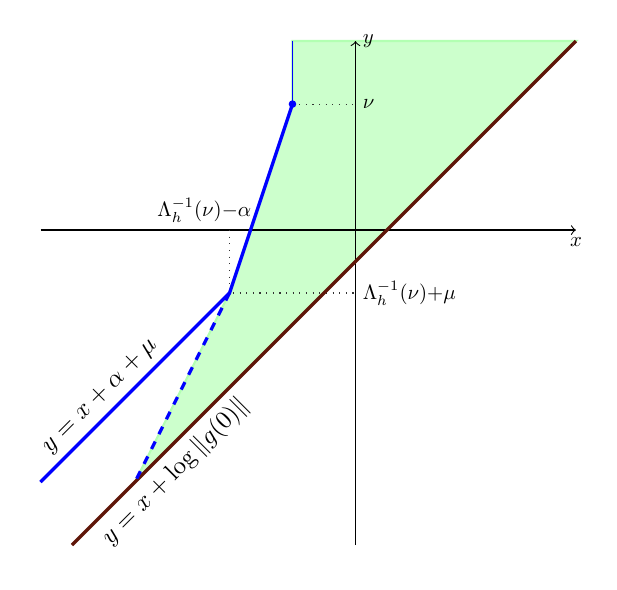
\begin{tikzpicture}[scale=0.8]
\draw[thick,green!30,fill=green!20] 
   (-2,-1)--(-1,2)--(-1,3)--(3.5,3)
 --(2.5,2)--(-3.5,-4)--cycle;
\draw[->] (-5,0)--(3.5,0);
\draw[->] (0,-5)--(0,3);
\node[below, scale=0.75] at (3.5,0) { $x$ };
\node[right, scale=0.75] at (0,3) { $y$ };
\draw[black!80,dotted] (-1,2)--(0,2);
\node[right,scale=0.75] at (0,2) { $\nu$ };
\draw[black!80,dotted] (-2,0)--(-2,-1)--(0,-1);
\node[above,scale=0.75] at (-2.4,0) { $\Lambda_h^{-1}(\nu){-}\alpha$ };
\node[right,scale=0.75] at (0,-1) { $\Lambda_h^{-1}(\nu){+}\mu$ };
\draw[Blue,very thick] (-5,-4)--(-2,-1)--(-1,2);
\fill[Blue] (-1,2) circle (0.06);
\draw[Blue] (-1,2)--(-1,3);
\draw[Sepia, very thick] (-4.5,-5)--(3.5,3);
\draw[Blue, very thick,dashed] (-2,-1)--(-3.5,-4);
\node[below right,rotate=45,scale=0.9] at (-4.3,-4.8) 
  { $y = x + \log \Vert g(0) \Vert$ };
\node[above right,rotate=45,scale=0.9] at (-4.8,-3.8) 
  { $y = x + \alpha + \mu$ };
\end{tikzpicture}
\hfill \null

\caption{Admissible region for the graph of $\Lambda(f)$}
\label{fig:area}
\end{figure}

Figure \ref{fig:area} illustrates Corollary \ref{cor:boundLambdaf}. The 
blue plain line represents the graph of the function $\Lambda_f$. A 
quick computation shows that, on a neighborhood of ${-}\infty$, this 
function is given by:
$$\Lambda_f(x) = x + \alpha + \mu$$
where $\mu$ is the value that $\Lambda_g$ takes on the interval 
$]{-}\infty, \nu]$. Corollary \ref{cor:boundLambdaf} says that the
graph of $\Lambda(f)$ lies below the plain blue line. We remark
moreover that the Taylor expansion of $f(x)$ starts with the term
$g(0) x$. Hence, on a neighborhood on ${-}\infty$, we have 
$\Lambda(f)(x) = x + \log \Vert g(0) \Vert$. Using convexity, we 
get:
$$\Lambda(f)(x) \geq x + \log \Vert g(0) \Vert, 
  \quad \forall x \in \R.$$
In other words, the graph of $\Lambda(f)$ lies above the brown line.
Furthermore, we know that the slopes of $\Lambda(f)$ are all integral
because $f$ is locally analytic. Hence, $\Lambda(f)$ cannot lie above
the dashed blue line defined as the line of slope $2$ passing through
the first break point of the blue plain line --- which has coordinate 
$(y_0 - \alpha - \mu, y_0)$ with $y_0 = \min(\Lambda_h^{-1}(\nu) + \mu, 
\nu)$. As a conclusion, we have proved that the graph of $\Lambda(f)$ 
must coincide with the brown line until it meets the dashed blue line 
and then has to stay in the green area.

As a consequence of the above discussion, we derive the following 
proposition which can be directly combined with Proposition 3.12 of 
\cite{padicprec}.

\begin{prop}
\label{prop:boundLambdaf2}
Keeping the above notations, we have:
$$\Lambda(f)_{\leq 2} (x) \leq 2(x + \alpha + \mu) -
\min(\Lambda_h^{-1}(\nu) + \mu, \: \nu)$$
for all $x \leq \min(\Lambda_h^{-1}(\nu) - \alpha, \: \nu - \mu - \alpha)$.
\end{prop}

\begin{proof}
Just remark that $y = 2(x + \alpha + \mu) - y_0$ is the equation of 
the dashed blue line.
\end{proof}

\noindent
\textbf{About the choice of the function $h$}

\smallskip

At the beginning of \S \ref{ssec:boundLambdaf}, we have introduced a 
function $h$ in our differential equation. The aim of this was to be 
more flexible and possibly get this way better bounds on $\Lambda(f)$. 
In this paragraph, we discuss a recommended choice for this function 
$h$.

Actually, we do recommend taking $h$ as the identity function 
\emph{but} changing the norm on the codomain of $h$ at the same time.
More precisely, if $F$ --- which is the $K$-Banach in which $f$ takes
its values --- is equipped with the norm $\Vert \cdot \Vert_F$, we 
recommand endowing it with the second norm defined by
$\Vert x \Vert'_F = \lambda \cdot \Vert x \Vert_F$ ($x \in F)$
where $\lambda$ is a positive real number that we shall choose later 
and taking $h : (F, \Vert \cdot \Vert_F) \to (F, \Vert \cdot \Vert'_F)$ 
acting as the identity on the underlying vector spaces. Doing this, the 
function $\Lambda(h)$ maps $x$ to $x + \log \lambda$ ($x \in \R$) and we 
choose $\Lambda_h = \Lambda(h)$.

We believe that a good way to optimize $\lambda$ is to choose it so that 
the two quantities in the minima in Proposition \ref{prop:boundLambdaf2} 
agree. With the expression we got just above for $\Lambda_h$, our 
heuristic yields $\log \lambda = \mu$, \emph{i.e.} $\lambda = e^\mu$.
Making this choice, the norms of $f(x)$ and $h(x)$ are comparable --- 
at least, on the domain we are interested in --- and we do not loose so 
much when we write that the norm of the couple $(f(x), h(x))$ is the 
maximum of those of $f(x)$ and $h(x)$.

{\color{Bittersweet}

\section{Univariate polynomials}
\label{sec:polynomials}

For any integer $d$, let us denote by $K_{< d}[X]$ the set of 
polynomials over $K$ of degree $< d$. It is a finite dimensional vector 
space of dimension $d$. The affine space $X^d + K_{< d}[X]$ is then 
the set of monic polynomials over $K$ of degree $d$. We denote it by 
$K_d[X]$.

\subsection*{Evaluation and interpolation.}

Beyond sums and products (which can be treated as before), two basic 
operations involving polynomials are evaluation and interpolation.
Evaluation models the function $(P,x) \mapsto P(x)$, where
$P$ is some polynomial and $x \in K$. Differentiating
it can be done by computing
\begin{equation}
\label{eq:diffeval}
(P + dP)(x + dx) = P(x + dx) + dP(x + dx) = P(x) + P'(x) dx + dP(x).
\end{equation}
Here $P'$ denotes the derivative of 
$P$. The differential at $P$ is then the linear map $(dP, dx) \mapsto 
P'(x) dx + dP(x)$.

As for interpolation, we consider a positive integer $d$ and the partial 
function $f : K^{2d} \to K_{< d}[X]$ which maps the tuple $(x_1, y_1, 
\ldots, x_d, y_d)$ to the polynomial $P$ of degree less than $d$ such 
that $P(x_i) = y_i$ for all $i$. The polynomial $P$ exists and is unique 
as soon as the $x_i$'s are pairwise distinct; the above function $f$ is 
then defined on this open set. Furthermore, if $(x_1, y_1, \ldots, x_d, 
y_d)$ is a point in it and $P$ denotes the corresponding interpolation 
polynomial, \eqref{eq:diffeval} shows that $d y_i = P'(x_i) dx_i + 
dP(x_i)$ for all $i$. For this, we can compute $dP(x_i)$ from $d x_i$ 
and $d y_i$ and finally recover $dP$ by performing a new interpolation.

\subsection*{Euclidean division.}

Let $A$ and $B$ be two polynomials with $B \neq 0$. The Euclidean division of 
$A$ by $B$ is the problem of finding $Q$ and $R$ with $A = BQ + R$ and $\deg R < \deg B$. 
Differentiating the above equality we find
\[
dA - dB \cdot Q = B \cdot dQ + dR,
\]
which implies that $dQ$ and $dR$ are respectively obtained as the 
quotient and the remainder of the Euclidean division of $dA - dB \cdot 
Q$ by $B$. This gives the differential. We note that the discussion 
above extends readily to convergent series (see also 
\cite{caruso-lubicz:14a}).

\subsection*{Greatest common divisors and B\'ezout coefficients.}

We fix two positive integers $n$ and $m$ with $n \geq m$. We consider the 
function $f : K_n[X] \times K_m[X] \to (K_{\leq n}[X])^3$ which sends a 
pair $(A,B)$ to the triple $(D, U, V)$ where $D$ is the \emph{monic} 
greatest common divisor of $A$ and $B$ and $U$ and $V$ are the B\'ezout 
coefficients of minimal degrees, computed by the extended 
Euclidean algorithm.
The nonvanishing of the resultant of $A$ and $B$ defines a Zariski open 
subset $\mathcal V_0$ where the function $\gcd$ takes the constant value 
$1$. On the contrary, outside $\mathcal V_0$, $\gcd(A,B)$ is a polynomial 
of positive degree.  Since $\mathcal V_0$ is dense, $f$ is not continuous outside 
$\mathcal V_0$. On the contrary, the function $f$ is differentiable, and even locally analytic,
on $\mathcal V_0$.

Of course, on $\mathcal V_0$, the first component $D$ is constant and 
therefore $dD = 0$. To compute $dU$ and $dV$, one can simply 
differentiate the B\'ezout relation $AU + BV = 1$. We get:
$$A \cdot dU + B \cdot dV = - (dA \cdot U + dB \cdot V)$$
from which we deduce that $dU$ (resp. $dV$) is obtained as the 
remainder in the Euclidean division of $U{\cdot}dX$ by $B$ (resp. of 
$V{\cdot}dX$ by $A$) where $dX = - (dA \cdot U + dB \cdot V)$.

In order to differentiate $f$ outside $\mathcal V_0$, we 
define the subset $\mathcal V_i$ of $K_n[X] \times 
K_m[X]$ as the locus where the $\gcd$ has degree $i$. The theory of 
subresultants shows that $\mathcal V_i$ is locally closed with respect to 
the Zariski topology. In particular, it defines a $K$-manifold in the 
sense of Appendix \ref{sec:manifold}, and the 
restriction of $f$ to $\mathcal V_i$ is differentiable. To compute
its differential, we proceed along the same lines as before: we 
differentiate the relation $AU + BV = D$ and obtain this way
$A \cdot dU + B \cdot dV - dD = dX$
with $dX = - (dA \cdot U + dB \cdot V)$. In the above relation, the
first two terms $A{\cdot}dU$ and $B{\cdot}dV$ are divisible by $D$ 
whereas the term $dD$ has degree less than $i$. 
Hence if $dX = D \cdot dQ + dR$ is the Euclidean division of $dX$ by $D$, 
we must have $\frac A D \cdot dU + \frac B D \cdot dV = dQ$ and $dD = 
-dR$. These relations, together with bounds on the degree of $U$ and $V$,
imply as before that $dU$ (resp. $dV$) are equal to the remainder in the
Euclidean division of $U{\cdot}dQ$ by $\frac B D$ (resp. of $V{\cdot}dQ$
by $\frac A D$).

\medskip

The lesson we may retain from this study is the following. If we have to 
compute the greatest common divisor of two polynomials $A$ and $B$ known 
with finite precision, we first need to determine what is its degree. 
However, the degree function is not continuous --- it is only upper 
semi-continuous --- and hence cannot be determined with certainty from $A$ and 
$B$, unless the approximation to $(A,B)$ lies entirely within $\mathcal V_0$.

We therefore need to make an extra hypothesis.  The most natural hypothesis to make
is that $\gcd(A, B)$ has the maximal possible degree.  The main reason for choosing
this convention is that if the actual polynomials $A, B \in K[X]$ have a greatest common
divisor of degree $i$ then there is some precision for which the maximal degree will be
equal to $i$, whereas if they have a positive
degree common divisor then no amount of increased precision will eliminate an intersection
with $\mathcal V_0$.  A second justification is that any other choice would yield a result
with no precision, since $A$ and $B$ appear to lie in $\mathcal V_i$ at the known precision.
Once this assumption is made, the computation is possible and one can apply Lemma 
\ref{lem:main} to determine the precision of the result.
Note that with the above convention, the $\gcd$ of $A$ and $A$ is $A$ 
itself although there exist pairs of coprime polynomials in any 
neighborhood of $(A,A)$.

\subsection*{Factorization.}

Suppose that we are given a polynomial $P_0 \in K_d[X]$ written as a 
product $P_0 = A_0 B_0$, where $A_0$ and $B_0$ are monic and coprime. 
Hensel's lemma implies that there exists a small neighborhood $\mathcal 
U$ of $P_0$ in $K_d[X]$ such that any $P \in \mathcal U$ factors 
uniquely as $P = A B$ with $A$ and $B$ monic and close enough to $A_0$ 
and $B_0$ respectively. Thus, we can consider the map $f : P 
\mapsto (A,B)$ defined on the subset of $\mathcal U$ consisting of monic 
polynomials. We want to differentiate $f$ at $P_0$. For this, we 
differentiate the equality $P = A B$ around $P_0$, obtaining
\begin{equation}
\label{eq:difffactor}
dP = A_0 \cdot dB + B_0 \cdot dA.
\end{equation}
where $dP$, $dA$ and $dB$ have degree less than $\deg P$, $\deg A$ and 
$\deg B$ respectively. If $A_0 U_0 + B_0 V_0 = 1$ is a Bezout relation
between $A_0$ and $B_0$, it follows from \eqref{eq:difffactor} that
$dA$ (resp. $dB$) is the remainder in the Euclidean division of $V_0
{\cdot} dP$ by $A_0$ (resp. of $U_0 {\cdot} dP$ by $B_0$).

\subsection*{Finding roots.}

An important special case of the previous study occurs when $A_0$ has 
degree $1$, that is $A_0(X) = X - \alpha_0$ with some $\alpha_0 \in K$. 
The map $P \mapsto A$ is then nothing but the mapping that 
follows the simple root $\alpha_0$. Of course, its differential around 
$P_0$ can be computed by the above method. Nevertheless, we may
obtain it more directly by expanding the equation $(P_0 + 
dP)(\alpha_0 + d\alpha) = 0$, obtaining
$P_0'(\alpha_0) d\alpha + dP(\alpha_0) = 0$.
Since $\alpha_0$ is a simple root, $P_0'(\alpha_0)$ 
does not vanish and we find:
$$d \alpha = - \frac{dP(\alpha_0)}{P'_0(\alpha_0)}.$$

We now address the case of a multiple root. Let $P_0$ be a monic 
polynomial of degree $d$ and $\alpha_0 \in K$ be a root of $P_0$ having 
multiplicity $m > 1$. Due to the multiplicity, it is no longer possible 
to follow the root $\alpha_0$ in a neighborhood of $P_0$. But it is if we 
restrict ourselves to polynomials which have a root of multiplicity $m$ 
close to $\alpha_0$. More precisely, let us consider the locus $\mathcal 
V_m$ consisting of monic polynomials of degree $d$ having a root of 
multiplicity at least $m$. It is a Zariski closed subset of $K_d[X]$ and
contains by assumption the polynomial $P_0$. 
Moreover, the irreducible components of $\mathcal V_m$ that meet at 
$P_0$ are in bijection with the set of roots of $P_0$ of multiplicity 
$\geq m$. In particular, $\alpha_0$ corresponds to one of these 
irreducible components; let us denote it by $\mathcal V_{m,\alpha_0}$. 
The algebraic variety $\mathcal V_{m,\alpha_0}$ is \emph{a fortioti} a
$K$-manifold. Moreover there exists a differentiable function $f$ which 
is defined on a neighborhood of $P_0$ in $\mathcal V_{m,\alpha_0}$ and 
follows the root $\alpha_0$, \emph{i.e.} $f(P_0) = \alpha_0$ and for all 
$P$ such that $f(P)$ is defined, $\alpha = f(P)$ is a root of 
multiplicity (at least) $m$ of $P$. The existence of $f$ follows from 
Hensel's Lemma applied to the factorisation $P_0(X) = (X-\alpha_0)^m 
B_0(X)$ where $B_0(X)$ is a polynomial which is coprime to $X - 
\alpha_0$. We can finally compute the differential of $f$ at $P_0$ 
(along $\mathcal V_{m,\alpha_0}$) by differentiating the equality
$P^{(m-1)}(\alpha) = 0$ where $P^{(i)}$ denotes the $i$-th derivative
of $P$. We find:
\begin{equation}
\label{eq:dalphamult}
d \alpha = - \frac{dP^{(m-1)}(\alpha_0)}{P_0^{(m)}(\alpha_0)}.
\end{equation}

The above computation has interesting consequences for $p$-adic 
precision. For example, consider the monic 
polynomial $P(X) = X^2 + O(p^{2N}) X + O(p^{2N})$ (where $N$ is some 
large integer) and suppose that we are asking a computer to compute one 
of its roots. What is the right answer? We remark that, if $\alpha$ is 
any $p$-adic number divisible by $p^N$, then $P(X)$ can be $X^2 - 
\alpha^2$ whose roots are $\pm \alpha$. Conversely, we can prove that 
the two roots of $P$ are necessarily divisible by $p^N$. Hence, the
right answer is certainly $O(p^N)$. Nevertheless, if we know in addition 
that $P$ has a double root, say $\alpha$, we can write $P(X) = (X - 
\alpha)^2$ and identifying the coefficient in $X$, we get $\alpha =
O(p^{2N})$ if $p > 2$ and $\alpha = O(p^{2N-1})$ if $p=2$.
This is exactly the result we get by applying Lemma \ref{lem:main} and
using \eqref{eq:dalphamult} to simplify the differential.

This phenomenon is general: if $P$ is a polynomial over $\Q_p$ known at 
some finite precision $O(p^N)$, a root $\alpha$ of $P$ having possibly 
multiplicity $m$ (\emph{i.e.} $P(\alpha), P'(\alpha), \ldots, P^{(m-1)} 
(\alpha)$ vanish at the given precision) can be computed at precision 
roughly $O(p^{N/m})$. However, if we know in advance that $\alpha$ has 
multiplicity $m$ then we can compute it at precision $O(p^{N-c})$ 
where $c$ is some constant (depending on $P$ and $\alpha$ but not on
$N$).

\section{Multivariate polynomials}

We consider the ring $K[\XX] = K[X_1, \ldots, X_n]$ of polynomials in $n$
variables over $K$ and fix a monomial order on it. 

\subsection*{Division.}

We then have a notion of division in $K[\XX]$: if $f, f_1, \ldots, f_s$ 
are polynomials in $K[\XX]$, then one may decompose $f$ as
$$f = q_1 f_1 + \cdots + q_s f_s + r$$
where $q_1, \ldots, q_s, r \in K[\XX]$ and no term of $r$ is divisible
by the leading term of some $f_i$ ($1 \leq i \leq s$). Moreover, assuming
that $(f_1, \ldots, f_s)$ is a Gr\"obner basis\footnote{A canonical choice of $r$ exists even without this
assumption. However, we do not know
if the computation of the differential that follows extends to this more
general setting.} of the ideal generated by these polynomials, the 
polynomial $r$ is uniquely determined and called the \emph{remainder} of 
the division of $f$ by the family $(f_1, \ldots, f_s)$. The map 
$(f, f_1, \ldots, f_s) \mapsto r$ is then well defined and we can compute its differential,
finding that $dr$ is obtained as the remainder of the division of $f - (q_1 
\cdot d f_1 + \cdots + q_s \cdot d f_s)$ by $(f_1, \ldots, f_s)$.

\subsection*{Gr\"obner basis.}

Recall that any 
ideal $I \subset K[\XX]$ admits a unique reduced Gr\"obner basis. We may
consider the map sending a family $(f_1, \ldots, f_s)$ of 
\emph{homogeneous}\footnote{This restriction will be convenient for us 
mainly because we are using the article \cite{vaccon:14a}, which deals only 
with homogeneous polynomials. It is however probably not essential.} 
polynomials of fixed degrees to the reduced Gr\"obner basis $(g_1, 
\ldots, g_t)$. It follows from \cite{vaccon:14a}*{Thm. 1.1} that this 
map is continuous at $(f_1, \ldots, f_s)$ provided that:
\begin{itemize}
\item the sequence $(f_1, \ldots, f_s)$ is regular
\item for all $i \in \{1, \ldots, s\}$, the ideal generated by
$f_1, \ldots, f_i$ is weakly-$w$ where $w$ denotes the fixed monomial
order (\emph{cf} \cite{vaccon:14a} for more detail).
\end{itemize}
A similar argument proves that it is actually differentiable at such
points. We are now going to compute the differential. For this we
remark that since the families $(f_1, \ldots, f_s)$ and $(g_1, \ldots,
g_t)$ generate the same ideal, we have a relation:
\begin{equation}
\label{eq:prodgrobner}
(g_1, \ldots, g_t) = (f_1, \ldots, f_s) \cdot A
\end{equation}
where $A$ is an $(s \times t)$ matrix with coefficients in $K[\XX]$.
Following Vaccon's construction, we see that the entries of $A$ 
can be chosen in such a way that they define differentiable functions.
Differentiating \eqref{eq:prodgrobner}, we get
$$(d g_1, \ldots, d g_t) =
(d f_1, \ldots, d f_s) \cdot A + (f_1, \ldots, f_s) \cdot dA.$$
Finally, since $(g_1, \ldots, g_t)$ is a \emph{reduced} Gr\"obner
basis, the above equality implies that $d g_i$ is the remainder in
the division of the $i$-th entry of the product
$(d f_1, \ldots, d f_s) \cdot A$ by the family $(g_1, \ldots, g_t)$.

\section{Matrices}
\label{sec:matrices}

Differentiating ring operations (sum, products, inverse) over matrices 
is again straightforward, keeping in mind that matrix algebras are not
commutative.

\subsection*{Determinants and characteristic polynomials.}

We first outline the standard computation of the differential of the function
$\det : M_n(K) \to K$. Suppose that $M \in \GL_n(K)$ and that $\com(M) = \det(M) M^{-1}$.
Then
\begin{align*}
\det(M + dM) &= \det(M) \cdot \det(I + M^{-1} \cdot dM)  \\
&= \det(M) \cdot \big(1 + \tr(M^{-1} \cdot dM)\big) \\
&= \det(M) + \tr(\com(M) \cdot dM).
\end{align*}
The differential of $\det$ at $M$ is then $dM \mapsto \tr(\com(M) \cdot dM)$. It turns
out that this formula is still valid when $M$ is not invertible.
The same computation extends readily to characteristic polynomials,
since they are defined as determinants. More precisely, let us 
consider the function $\chi : M_n(K) \to K_n[X]$ taking a matrix 
$M$ to its monic characteristic polynomial $\det(X-M)$.
Then $\chi$ is differentiable at each point $M \in M_n(K)$ and its 
differential is given by $dM \mapsto \tr(\com(X{-}M) \cdot dM)$.

\subsection*{LU factorization.}

Define the LU factorization of a square matrix $M \in M_n(K)$ as a decomposition $M = LU$ 
where $L$ is lower triangular and unipotent and $U$ is upper triangular. 
Such a decomposition exists and is unique provided that no principal minor
of $M$ vanishes. We can then consider the mapping $M \mapsto (L,U)$ 
defined over the Zariski-open set of matrices satisfying the above 
condition. In order to differentiate it, we differentiate the relation 
$M = LU$ and rewrite the result as
$$L^{-1} dM \: U^{-1} = L^{-1} \cdot dL + dU \cdot U^{-1}.$$
We remark that in the right hand side of the above formula, the first
summand is lower triangular with zero diagonal whereas 
the second summand is upper triangular. Hence in order to compute $dL$
and $dU$, one can proceed as follows: 
\begin{enumerate}
\item compute the product $dX = L^{-1} dM \: U^{-1}$,
\item separate the lower and upper part of $dX$ obtaining $L^{-1} \cdot dL$ and $dU \cdot U^{-1}$
\item recover $dL$ and $dU$ by multiplying the above matrices by $L$ on the left and $U$ on the right respectively.
\end{enumerate}
The above discussion extends almost \emph{verbatim} to LUP 
factorization; the only difference is that LUP factorizations are not 
unique but they are on a small neighborhood of $M$ if we fix the matrix 
$P$.

\subsection*{QR factorization.}

A QR factorization of a square matrix $M \in M_n(K)$ will be
a decomposition $M = QR$ where $R$ is unipotent upper triangular and $Q$ is
orthogonal in the sense that $\trans Q \cdot Q$ is diagonal. As before, such 
a decomposition exists and is unique on a Zariski-open subset of $M_n(K)$. The
mapping $f : M \mapsto (Q,R)$ is then well defined on this subset. We 
would like to emphasize at this point that the orthogonality condition
defines a sub-manifold of $M_n(K)$ which is \emph{not} a
vector space: it is defined by equations of degree $2$. The codomain
of $f$ is then also a manifold; this example then fits into the setting
of Appendix \ref{sec:manifold} but not to those of Section \ref{sec:mainlemma}. 
We can differentiate $f$ by following the method used for LU 
factorization.  Differentiating the relation $M = QR$, we obtain
\begin{equation}
\label{eq:diffQR}
\trans Q \cdot dM \cdot R^{-1} = \trans Q \cdot dQ + \Delta \cdot dR 
\cdot R^{-1}
\end{equation}
where $\Delta = \trans Q \cdot Q$ is a diagonal matrix by definition.
Moreover by differentiating $\trans Q \cdot Q = \Delta$, we find that
$\trans Q \cdot dQ$ can be written as the sum of an antisymmetric 
matrix and a diagonal one. Since moreover $dR \cdot R^{-1}$ is upper
triangular with all diagonal entries equal to $0$, we see that 
\eqref{eq:diffQR} is enough to compute $dQ$ and $dR$ from $Q$, $R$ 
and $dM$.

\section{Vector spaces}

In computer science, vector spaces are generally represented as subspaces 
of $K^n$ for some $n$. Hence they naturally appear as points on some 
grassmannian $\Grass(n,d)$. These grassmannians are $K$-manifolds in the 
sense of Appendix \ref{sec:manifold} as it is discussed in \S 
\ref{sec:exmanifold}. In the sequel, we use freely the formalism 
introduced there.

\subsection*{Left kernels.}

Let $d$ and $n$ be two nonnegative integers such that $d \leq n$.
We consider the open subset $\mathcal V_{n-d}$ of $M_{n,n-d}(K)$ 
consisting of matrices of full rank, \emph{i.e.} rank $n-d$. The left 
kernel defines a mapping $\text{LK} : M_{n,n-d}(K) \to \Grass(d,n)$. Let 
us prove that it is differentiable and compute its differential around 
some point $M \in M_{n,n-d}(K)$. Of course, there exists a neighborhood 
$\mathcal U$ of $M$ whose image is entirely contained in a given chart 
$U_P$. We assume for simplicity that $P$ is the identity. On $\mathcal 
U$, the map $\text{LK}$ corresponds in our chart to the map that 
takes $M$ to the unique matrix $N \in M_{d, n-d}(K)$ such that 
$\begin{pmatrix} I_d & N \end{pmatrix} \cdot M = 0$. The implicit 
function theorem then implies that $\text{LK}$ is differentiable. 
Furthermore, its differential satisfies the relation
$\begin{pmatrix} 0 & dN \end{pmatrix} \cdot M +
\begin{pmatrix} I_d & N \end{pmatrix} \cdot dM = 0$,
from which we can compute $dN$ by projecting on the $(n-d)$ last
columns.

Following what we have already done in \S \ref{sec:polynomials} for 
greatest common divisors of polynomials, we can develop further this 
example and study what happens on the closed subset of $M_{n,n-d}(K)$ 
where matrices have not full rank. On this subspace, the left kernel has 
dimension $< d$ and then no longer defines a point in $\Grass(n,d)$. 
Nevertheless, for all integer $r < n-d$, we can consider the subset 
$\mathcal V_r \subset M_{n,n-d}(K)$ of matrices whose rank are exactly 
rank $r$. It is locally closed in $M_{n,n-d}(K)$ with respect to the 
Zariski topology and hence defines a $K$-manifold. Furthermore, we have a 
mapping $\text{LK}_r : \mathcal M_r \to \Grass(n,n-r)$ which is 
differentiable and whose differential can be computed as before.

\subsection*{Intersections.}

We pick $n$, $d_1$ and 
$d_2$ three nonnegative integers such that $d_1 \leq n$, $d_2 \leq n$ 
and $d_1 + d_2 \geq n$. Two subspaces of $K^n$ of dimension $d_1$ and 
$d_2$ respectively meet along a subspace of dimension at most $d_1 + d_2 
- n$. For all $d \leq d_1 + d_2 -n$, we can then define the subspace 
$\mathcal V_d$ of $\Grass(n,d_1) \times \Grass(n,d_2)$ consisting of 
pairs $(E_1, E_2)$ such that $\dim (E_1 \cap E_2) = d$ and consider the 
function $f_d : \mathcal V_d \to \Grass(n, d)$ which sends $(E_1, E_2)$ 
to $E_1 \cap E_2$. In charts, the function $f_d$ can be interpreted as
the kernel of a matrix simply because $E_1 \cap E_2$ appears as the
kernel of the canonical linear map $E_1 \oplus E_2 \to K^n$. We thus deduce
that $f_d$ is differentiable and that its differential can be
computed as above.

\subsection*{Sums and images.}

Finally, we note that similar results hold for images of matrices and,
consequently, sums of subspaces.

}

%\bibliographystyle{plain}
%\bibliography{roebib/Biblio,extras}

\end{document}
